% Resultados -- RQ 05 e RQ 06 (parte do Arthur).
% Números de resultados/rq5_spearman.csv e resultados/rq6_testes.csv.

\subsection{RQ 05: frequência de deploy e taxa de falha}

Calculamos a correlação de Spearman entre a frequência de \textit{deploy} e o CFR,
separadamente para cada variante. Spearman trabalha com postos, o que é adequado às
distribuições assimétricas observadas e ao grande número de empates em zero no CFR (a).

\begin{table}[ht]
\centering
\caption{Correlação entre frequência de \textit{deploy} e CFR, por variante.}
\label{tab:rq5}
\begin{tabular}{lrrrl}
\hline
\textbf{Variante do CFR} & \textbf{n} & $\boldsymbol{\rho}$ & \textbf{p} & \textbf{Interpretação} \\
\hline
(a) proxy de CI      & 350 & 0,127 & 0,017   & fraca positiva \\
(b) proxy de entrega & 350 & 0,613 & $<$ 0,001 & forte positiva \\
\hline
\end{tabular}
\end{table}

As duas são estatisticamente significativas ao nível de 5\%, mas o coeficiente da variante (b)
é quase cinco vezes o da (a). Na variante (a), um $\rho$ de 0,127 explica menos de 2\% da variância
conjunta: na prática, frequência de publicação e falha de CI são independentes nesta amostra.
Na variante (b), o $\rho$ de 0,613 indica associação forte. A Figura~\ref{fig:rq5} mostra as
duas dispersões, com a frequência em escala logarítmica.

\begin{figure}[ht]
\centering
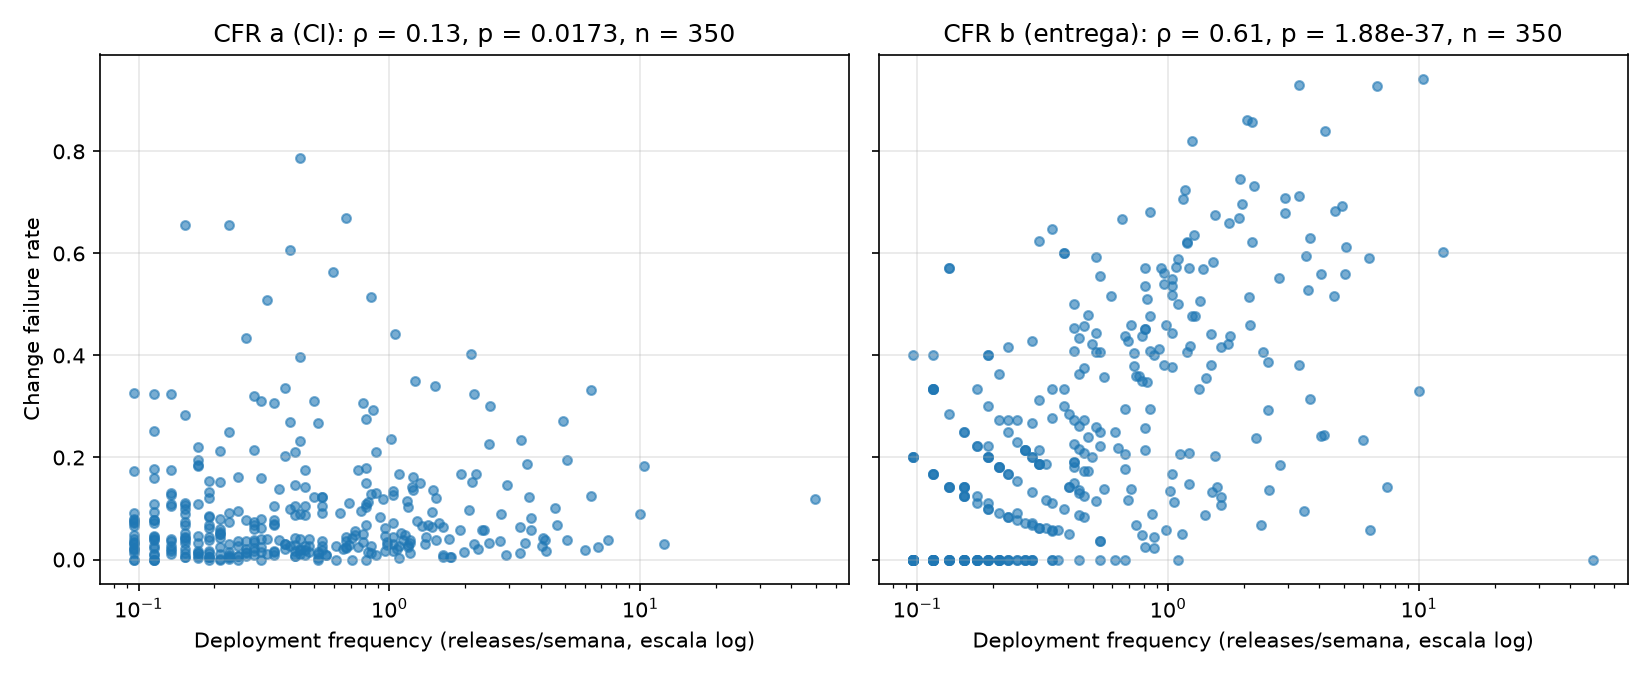
\includegraphics[width=\textwidth]{rq5_dispersao.png}
\caption{Frequência de \textit{deploy} (escala log) contra o CFR, nas duas variantes.}
\label{fig:rq5}
\end{figure}

\subsection{RQ 06: fatores associados ao desempenho}

Comparamos cada métrica entre subgrupos de cinco fatores: linguagem (as cinco mais frequentes,
e ``Outras''), quartis de estrelas, quartis de contribuidores, quartis de idade e tipo do
projeto. Usamos Kruskal-Wallis para três ou mais grupos e Mann-Whitney para dois, com
$\varepsilon^2$ e Cliff's delta como tamanho de efeito. Como são 30 testes simultâneos,
aplicamos a correção de Holm~\cite{holm1979} sobre o conjunto.

Doze dos 30 testes permanecem significativos após a correção (Tabela~\ref{tab:rq6}).

\begin{table}[ht]
\centering
\caption{Testes significativos após a correção de Holm, ordenados pelo tamanho de efeito.}
\label{tab:rq6}
\begin{tabular}{llrr}
\hline
\textbf{Fator} & \textbf{Métrica} & \textbf{p (Holm)} & $\boldsymbol{\varepsilon^2}$ \\
\hline
Idade          & Lead time (a) & $<$ 0,001 & 0,288 \\
Idade          & Lead time (b) & $<$ 0,001 & 0,251 \\
Contribuidores & Lead time (b) & $<$ 0,001 & 0,171 \\
Idade          & CFR (b)       & $<$ 0,001 & 0,164 \\
Idade          & Frequência    & $<$ 0,001 & 0,106 \\
Contribuidores & Lead time (a) & $<$ 0,001 & 0,104 \\
Linguagem      & Lead time (a) & $<$ 0,001 & 0,099 \\
Linguagem      & Frequência    & $<$ 0,001 & 0,097 \\
Linguagem      & CFR (b)       & $<$ 0,001 & 0,084 \\
Linguagem      & Lead time (b) & 0,001     & 0,078 \\
Idade          & Recuperação   & 0,016     & 0,051 \\
Estrelas       & Lead time (b) & 0,014     & 0,049 \\
\hline
\end{tabular}
\end{table}

Por fator, a idade aparece em cinco métricas, a linguagem em quatro, os contribuidores em
duas e as estrelas em uma. Nenhum teste sobre o tipo do projeto sobreviveu à
correção, e esse fator só existe para os 60 repositórios da amostra-ouro, de modo que os
testes sobre ele têm poder reduzido.

Entre os testes significativos, $\varepsilon^2$ vai de 0,049 a 0,288; o maior corresponde à
idade sobre o \textit{lead time} (a). Nenhum fator isolado explica a maior
parte da variação observada.
